\documentclass{llncs}

\usepackage[T1]{fontenc}
\usepackage{inconsolata}
\usepackage[polish]{babel}
\usepackage[utf8]{inputenc}
\usepackage{listings}
\usepackage{color}
\usepackage{enumerate}

\definecolor{pblue}{rgb}{0.13,0.13,1}
\definecolor{pgreen}{rgb}{0,0.5,0}
\definecolor{pred}{rgb}{0.9,0,0}
\definecolor{pgrey}{rgb}{0.46,0.45,0.48}

\usepackage{graphicx}
\usepackage{listings}
\lstset{language=Java,
  showspaces=false,
  showtabs=false,
  breaklines=true,
  showstringspaces=false,
  breakatwhitespace=true,
  commentstyle=\color{pgreen},
  keywordstyle=\color{pblue},
  stringstyle=\color{pred},
  basicstyle=\ttfamily\small,
}

\lstset{
  literate={ą}{{\k{a}}}1
           {ć}{{\'c}}1
           {ę}{{\k{e}}}1
           {ó}{{\'o}}1
           {ń}{{\'n}}1
           {ł}{{\l{}}}1
           {ś}{{\'s}}1
           {ź}{{\'z}}1
           {ż}{{\.z}}1
           {Ą}{{\k{A}}}1
           {Ć}{{\'C}}1
           {Ę}{{\k{E}}}1
           {Ó}{{\'O}}1
           {Ń}{{\'N}}1
           {Ł}{{\L{}}}1
           {Ś}{{\'S}}1
           {Ź}{{\'Z}}1
           {Ż}{{\.Z}}1
}


\begin{document}


\title{Opracowanie i implementacja podstaw optymalnego przechowywania i transferowania danych medycznych (ontologie)}

\author{Patryk Bąk, Marek Kendziorek, Wojciech Inglot}

\institute{AGH Kraków, 2013}
\maketitle


\section{Abstrakt}
\label{sec:Abstrakt}

Systemy medyczne należą do jednych z najbardziej rozbudowanych systemów w branży IT. Cechują się one nie tylko ogromnymi ilosciami danych, które przetwarzają, ale również bardzo dużą złożonoscią budowych tych danych oraz relacji, które między nimi zachodzą. Własnie branża e-health jako jedna z pierwszych zainteresowała się zastosowaniem ontologii oraz ich reprezentacji w zagadnieniu reprezentowania danych. Niniejszy artykuł porusza problem zastosowania optymalnych technologii i metodologii do implementacji systemu opartego o ontologię z naciskiem na przechowywanie oraz transfer ontologii.

Zaproponowane przez nas rozwiązanie problemu oparte zostało na języku programowania java oraz opartych na nim technologiach i narzędziach. Do transferu danych wykorzystano FUSEKI, które oferuje transfer danych protokołem REST z wykorzystaniem języka zapytań SPARQL. Dodatkowo przy definiowanu ontologii zaproponowano wykorzystanie opartego i interfejsy i stałe słownika danych.

Zaproponowana przez nas implementacja reprezentacji oraz transferu danych medycznych posiada wiele cech pożądanych przy projektowaniu tego typu systemów. Rozwiązanie to cechuje się bardzo dużą skalowalnoscią zarówno od strony wielkosci samego systemu jak i możliwosci rozbudowy przechowywanych w nim danych. Zastosowanie architektury typu SOA przy budowie systemu medyczneo pozwala na łatwą, modułową rozbudowę takiego systemu oraz ułatwioną integrację z innymi systemami medycznymi, zupełnie niezależnymi od siebie.



\begin{multicols}{2}
\section{Wstep}
\label{cha:wstep}

\subsection{Ontologia}
\label{sec:ont}

\subsection{OWL}
\label{sec:owl}

OWL (Ontology Web Language) jest opartym na składni XML językiem służącym do opisu ontologii. Stanowi on rozszerzenie języka RDF (Resource Definition Language). Istnieją 3 odmiany OWL: OWL Lite, OWL DL oraz OWL Full. W 2004 roku język ten został uznany za standard przez organizację W3C.

OWL został stworzony do przetwarzania informacji o obiektach oraz relacji między nimi, nie do przechowywania tych informacji w formie czytelnej dla człowieka. OWL jest zbudowany na bazie RDF, tak więc języki te są ze sobą w pełni kompatybilne. OWL posiada jednak znacznie mocniejszą składnię.

Do elementów języka OWL należą takie atrybuty jak:

\begin{itemize}

\item Class - definiuje grupę indywidualnosci, które posiadają pewne wspólne cechy. Klasy można organizować w hierarchie za pomocą atrybutu subClassOf.


\item rdf:Property - okresla pewne relacje między indywidualnosciami np. samochod może posiadać drzwi, osoba moze posiadać dziecko albo rodzica.

\item rdfs:domain - ogranicza indywidualności, do których można zastosować relację (property). Jeżeli relacja łączy jedną indywidualność z drugą, i jednocześnie posiada ona domenę na określoną klasę, to obie indywidualności muszą należeć do tej klasy.

\item rdfs:range - ogranicza nie tylko indywidualności, ale także wartość relacji (property)

\item Individual - indywidualności są instancjami klas, które są połączone pewnymi relacjami (property).

\end{itemize}

Wszystkie powyższe atrybuty są częścią specyfikacji OWL Lite.



\subsection{SPARQL}
\label{sec:sparql}

\subsection{REST}
\label{sec:rest}

REST jest protokołem komunikacji między aplikacjami, który tak naprawdę jest tylko pewną dodatkową warstwą nałożoną na protokół HTTP. Budowanie zapytań restowych z poziomu języków programowania jest tak samo proste, jak zrozumienie działania protokołu HTTP. Istnieje wiele bibliotek i prostych frameworków do budowania serwisów, odbierających i wysyłających zapytania HTTP. Należą do nich np Jersey-RS, czy zbudowana na jego bazie trochę większa biblioteka Apache CXF. Biblioteka Fuserki, będąca częścią specyfikacji Apache Jena oferuje możliwość transferu danych właśnie protokołem REST, przy użyciu języka zapytań SPAQRL. 

Ze względu na swoją prostotę i oparcie o standard HTT, wybór tego protokołu jako sposobu komunikacji między aplikacjami jest bardzo dobrą decyzją. Umożliwia to znakomitą skalowalność naszego systemu, poprzez rozdzielenie go na szereg indywidualnych aplikacji, które nie muszą być napisane przy użyciu tej samej technologii, muszą jedynie współdzielić tą metodę komunikacji oraz ewentualnie sposób serializacji danych.


\section{Wykorzystane technologie}
\label{cha:technologie}

\subsection{Ontologia}
\label{sec:ont}

Ontologia jest formalną reprezentacją pewnej dziedziny wiedzy. Składają się na nią zapis zbiorów pojęć i relacji między nimi. Zapis ten tworzy schemat pojęciowy, który jest opisem danej dziedziny wiedzy. Może służyć jednocześnie jako podstawa do wnioskowania o właściwości opisywanych ontologią pojęć.	 \cite {7}

Pod pojęciem ontologii mogą się kryć różne struktury wiedzy. Ich przeznaczenie czy zakres stosowania może być wieloraki.

Ontologie możemy podzielić ze względu na stopień ich formalizacji:
\begin{itemize}
\item nieformalne
	\begin{itemize}
		\item predefiniowane słownictow
		\item słowniki
		\item tezarusy
		\item taksonomie
	\end{itemize}
\item formalne
	\begin{itemize}
		\item ontologie oparte na danych
		\item ontologie oparte na logice
	\end{itemize}
\end{itemize}

Podział następuje także ze względu na zakres stosowania:
\begin{itemize}
\item ontologie wysokiego poziomu (\textit{upper ontologies})
\item ontologie dziedzinowe (\textit{domain ontologies})
\item ontologie aplikacyjne
\end{itemize}

Istnieje szereg języków pozwalających na zapis lub wspierających ontologie:
\begin{itemize}
\item OWL (\textit{Ontology Web Language})
\item RDF (\textit{Resource Description Framework})
\item RDF Vocabulary Description Language (RDF Schema, RDFS)
\item OCML (Operational Conceptual Modeling Language)
\item XML (Extensible Markup Language)
\end{itemize}

\subsection{OWL}
\label{sec:owl}

OWL (Ontology Web Language) jest opartym na składni XML językiem służącym do opisu ontologii. Stanowi on rozszerzenie języka RDF (Resource Definition Language). Istnieją 3 odmiany OWL: OWL Lite, OWL DL oraz OWL Full. W 2004 roku język ten został uznany za standard przez organizację W3C. \cite {8}

OWL został stworzony do przetwarzania informacji o obiektach oraz relacji między nimi, nie do przechowywania tych informacji w formie czytelnej dla człowieka. OWL jest zbudowany na bazie RDF, tak więc języki te są ze sobą w pełni kompatybilne. OWL posiada jednak znacznie mocniejszą składnię.

Do elementów języka OWL należą takie atrybuty jak:

\begin{itemize}

\item Class - definiuje grupę indywidualnosci, które posiadają pewne wspólne cechy. Klasy można organizować w hierarchie za pomocą atrybutu subClassOf.


\item rdf:Property - okresla pewne relacje między indywidualnosciami np. samochod może posiadać drzwi, osoba moze posiadać dziecko albo rodzica.

\item rdfs:domain - ogranicza indywidualności, do których można zastosować relację (property). Jeżeli relacja łączy jedną indywidualność z drugą, i jednocześnie posiada ona domenę na określoną klasę, to obie indywidualności muszą należeć do tej klasy.

\item rdfs:range - ogranicza nie tylko indywidualności, ale także wartość relacji (property)

\item Individual - indywidualności są instancjami klas, które są połączone pewnymi relacjami (property).

\end{itemize}

Wszystkie powyższe atrybuty są częścią specyfikacji OWL Lite.

\subsection{Protege}
\label{sec:protege}
Protege jest otwarto-źródłowym narzędziem stworzonym przez Stanford Medical Informatics \cite{26}. Jak przy większości narzędzi modelujących, architektura Protege jest przejrzyście podzielona na dwie części - model i widok. Modele są wewnętrzną reprezentacją mechanizmy ontologii i baz wiedzy. Widoki zapewniają interfejs użytkownika, dzięki któremu można wyświetlać i manipulować modelami.

Protege posiada możliwość wczytania, edycji i zapisywania w wielu popularnych dla ontologii formatach, np:
\begin{itemize}
\item RDF
\item OWL
\item XML
\item UML
\item Bazy relacyjne
\end{itemize}

\subsection{SPARQL}
\label{sec:sparql}

~SPARQL jest językiem zapytań RDF, czyli pozwala na wyciaganie lub manipulowanie danymi w bazie danych składującej dane w formacie RDF (eng. Resource Description Framework). SPARQL pozwala również na pracę na danych w formacie pochodnym od formatu RDF, np. OWL, jednak z pewnymi ograniczeniami. SPARQL operując na danych w formacie OWL musi pominąć elementy języka które nie mają przełożenia na format RDF.

~Konstrukcja zapytań opiera się o zestaw trzech parametrów:
\begin{itemize}
\item spójnika (eng. conjuction)
\item alternatywy (eng. disjunction)
\item wzorzec (opcjonalnie) (eng. pattern)
\end{itemize}

Idea jaka przyświecała twórcom SPARQL określała go jako przełom w tworzeniu internetu czytelnego dla maszyn. Jeżeli format ten przyjmie się jako standard otrzymamy uniwersalny sposób otrzymywania informacji z internetowych \quotedblbase skupisk\textquotedblright  danych, co da nowe możliwości łączenia danych z różnych źródeł.


\subsection{REST}
\label{sec:rest}

REST jest protokołem komunikacji między aplikacjami, który tak naprawdę jest tylko pewną dodatkową warstwą nałożoną na protokół HTTP. Budowanie zapytań restowych z poziomu języków programowania jest tak samo proste, jak zrozumienie działania protokołu HTTP. Istnieje wiele bibliotek i prostych frameworków do budowania serwisów, odbierających i wysyłających zapytania HTTP. Należą do nich np Jersey-RS, czy zbudowana na jego bazie trochę większa biblioteka Apache CXF. Biblioteka Fuserki, będąca częścią specyfikacji Apache Jena oferuje możliwość transferu danych właśnie protokołem REST, przy użyciu języka zapytań SPAQRL.  \cite{1}

Ze względu na swoją prostotę i oparcie o standard HTTP, wybór tego protokołu jako sposobu komunikacji między aplikacjami jest bardzo dobrą decyzją. Umożliwia to znakomitą skalowalność naszego systemu, poprzez rozdzielenie go na szereg indywidualnych aplikacji, które nie muszą być napisane przy użyciu tej samej technologii, muszą jedynie współdzielić tą metodę komunikacji oraz ewentualnie sposób serializacji danych.

\subsection{Fuseki}
\label{sec:rest}

~Fuseki jest to serwer HTTP w standardzie REST przyjmujący zapytania HTTP zawierające w parametrach zapytania SPARQL.
Dzięki niemu możemu w ustandaryzowany sposób pobierać lub manipulowac danymi w modelu OWL lub RDF.

~Fuseki jest jednym z subsystemów systemu Jena. Twórcy zadbali o to żeby serwer SPARQL udało się włączyć nie tylko poprzez konsole, ale również bezpośrednio z aplikacji JAVA z wykorzystaniem biblioteki Jena.

\subsection{HL7}
\label{sec:hl7}

HL7 (Health Level 7) jest organizacją ustanawiającą standardy, akredytowaną przez American National Standards Insitute (ANSI). Opracowali protokół komunikacyjny szeroko używany w USA, obecnie coraz częściej rozpoznawany i wykorzystywany w pozostałych częściach świata. \cite {14}

RIM (Reference Informational Model) został wykorzystany w trzeciej wersji HL7 (HL7 Version 3) w celu standaryzacji powiązań pomiędzy danymi przenoszonymi przez wiadomości protokołu HL7. \cite {16}

Diagram UML na rysunku \ref{fig:hl7rim} przedstawia podstawowe klasy istniejące w RIM. \cite {15}

RIM opiera się na pięciu podstawowych założeniach:
\begin{itemize}
	\item Każde zdarzenie jest opisane przez klasę Act
	\begin{itemize}
		\item zdarzeniem może być: procedura, obserwacja, dostawa zapasów, rejestracja, itp.
	\end{itemize}
 	\item Relacje pomiędzy zdarzeniami opisuje klasa ActRelationship
 	\item Klasa Participation definiuje kontekst wystąpienia zdarzenia
 	\begin{itemize}
 		\item autor, wykonujący, podmiot, lokalizacja itp.
 	\end{itemize}
 	\item uczestnicy zdarzenia są opisanie przez klasę Role
 	\begin{itemize}
 		\item pacjent, dostawca, praktykant, pracownik itp.
 	\end{itemize}
  	\item role są reprezentowane przez klasę Entity
  	\begin{itemize}
 		\item osoby, organizacja, materiały, miejsca, urządzenia, itp.
 	\end{itemize}
\end{itemize}

\end{multicols}
\begin{figure}[h]
	\center
	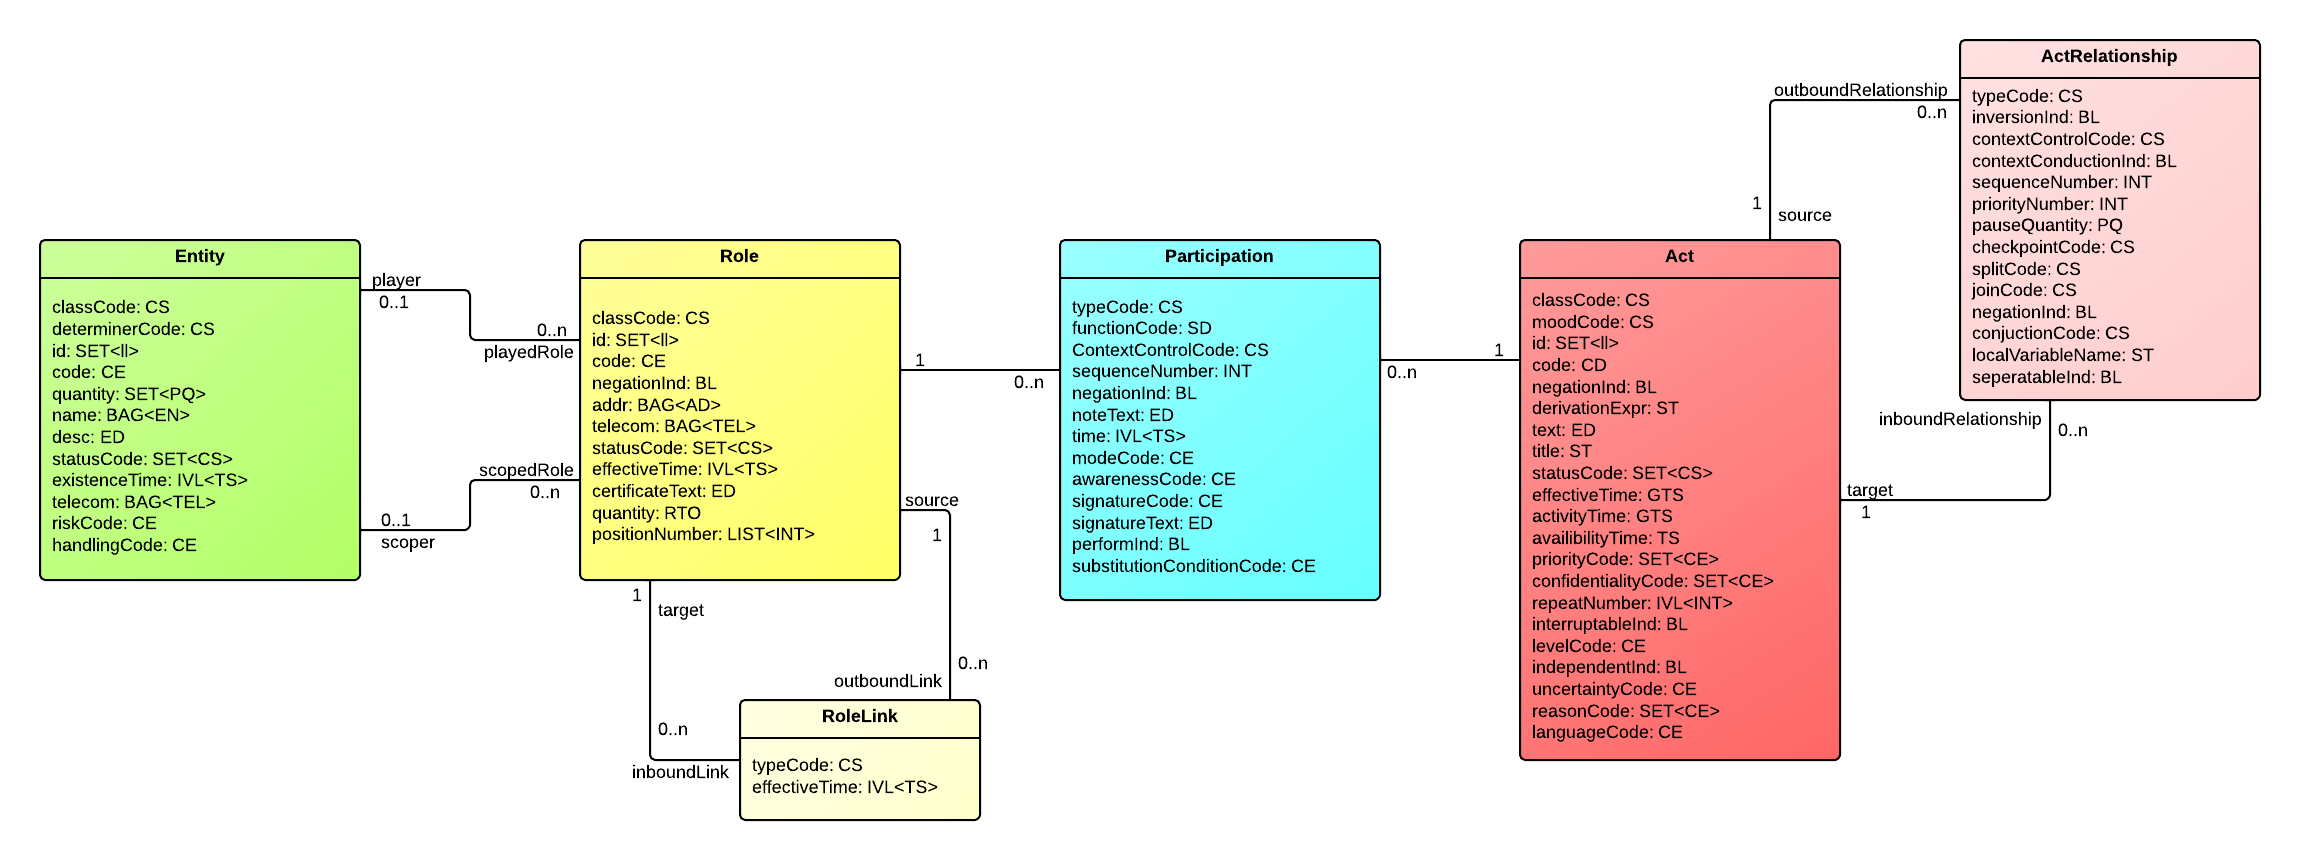
\includegraphics[width=\textwidth, scale=0.5]{pics/HL7}
	\caption{HL7 RIM}
	\label{fig:hl7rim}
\end{figure}
\begin{multicols}{2}
\section{Implementacja rozwiązania}
\label{cha:impl}

Rozwiązanie zaprezentowane w niniejszym artykule zostało napisane w języku Java, z wykorzystaniem Ontology API biblioteki Apache Jena. Biblioteka ta pozwala na mapowanie różnego rodzaju reprezentacji ontologii na klasy Java. Do transferowania naszych danych wykorzystamy bibliotekę Apache CXF, a dokładniej jej moduł REST, który pozwoli nam na przesyłanie zserializowanych danych przez protokół HTTP.

\subsection{Reprezentacja danych}
\label{sec:persist}

Ontology API biblioteki Apache Jena pozwala między innymi na budowanie oraz importowanie modeli ontologii. Stworzenie nowego modelu ontologii oraz zaimportowanie do niego już istniejącej ontologii zapisanej w formacie OWL przedstawiono na rysunku.

\end{multicols}
\newpage
\begin{figure}[p]
	\centering
	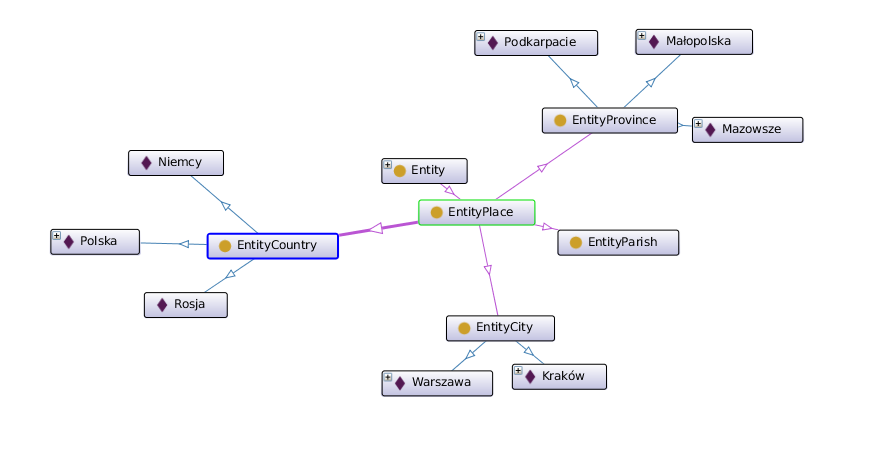
\includegraphics[scale=0.7, angle=90]{pics/EntityPlaceOntology}
	\caption{Przykład Ontologii Opartej o HL7 (EntityPlace)}
	\label{fig:placeont}
\end{figure}
\begin{figure}[p]
	\centering
	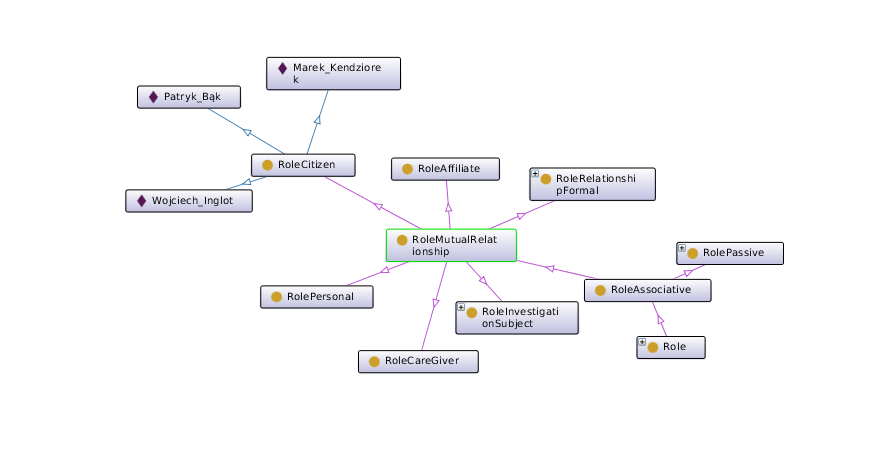
\includegraphics[scale=0.7, angle=90]{pics/RoleOntology}
	\caption{Przykład Ontologii Opartej o HL7 (Role)}
	\label{fig:placeont}
\end{figure}
\newpage
\begin{multicols}{2}

\subsection{Transfer danych}
\label{sec:transfer}

W projekcie uruchomiony został serwer HTTP Fuseki. Pozwala on na przechowywanie i udostepnienie danych wczytanych z plikow OWL poprzez zapytania HTTP. W jego wewnętrznej bazie danych budowane są grafu do których aplikacje klienckie odwołują się w zapytania SPARQL.

\subsubsection{Instalacja}

~Instalacja Jeny i Fuseki ogranicza się do dodania do zmiennych środowiskowych ścieżek do paczek.
\begin{lstlisting}
export JENA= /Users/XXXX/Fuseki/apache-jena-2.11.0/
export FUSEKI= /Users/XXXX/Fuseki/jena-fuseki-1.0.0/
\end{lstlisting}

\subsubsection{Uruchomienie serwera}

~Standardowo serwer FUSEKI uruchamiany jest pod wirtualną domeną \quotedblbase localhost\textquotedblright i na porcie 3030.

Uruchomienie serwera FUSEKI:
\begin{lstlisting}
./fuseki-server --update --loc=/Users/~/MyTDB/ /ds &
\end{lstlisting}

\subsubsection{Załadowanie pliku z ontologią}

~Załadowania pliku OWL (poprzez konsolową komendę):

\begin{lstlisting}
./s-put http://localhost:3030/ds/data default /Users/XXXX/RIMV3OWL.owl
\end{lstlisting}

\subsubsection{Tworzenie zapytania SPARQL}

~Wysłanie zapytania SPARQL wypisującego \quotedblbase koncepty\textquotedblright z załadowanego grafu:

\begin{enumerate}
\item Tworzenie zapytania.
\begin{lstlisting}
select distinct ?Concept where {[] a ?Concept}
\end{lstlisting}
\item Tworzenie zapytania HTTP POST, gdzie:
\begin{itemize}
\item jako URI podajemy sufix prowadzący do punktu końcowego (eng. endpoint) i doklajemy końcówkę /query
\item w parametrze POST/GET \quotedblbase query\textquotedblright podajemy stworzone zapytanie 
\item opcjonalne parametry: output (np. \quotedblbase json\textquotedblright ), default-graph-uri
\end{itemize}
\item W efekcie otrzymujemy zapytanie (dla punktu końcowego \quotedblbase ds\textquotedblright :
\end{enumerate}

\begin{lstlisting}
http://localhost:3030/ds/sparql? query=select+distinct++%3FConcept +where+%7B%5B%5D+a+%3FConcept%7D &default-graph-uri= &output=json
\end{lstlisting}
\section{Przypadek użycia}
\label{cha:usecase}

Zaprojektowany system będzie wykorzystywany w sposób pokazany na Rys. \ref{fig:usecase}. Celem implementacji jest stworzenie działającego przypadku użycia \quotedblbase Pobranie informacji o pacjencie\textquotedblright, który będzie wykorzystywany przez więcej niż jednego  \quotedblbase aktora (Doktor)\textquotedblright, a dane będą składowane w centralnej bazie.

\end{multicols}
\begin{figure}[h]
	\centering
	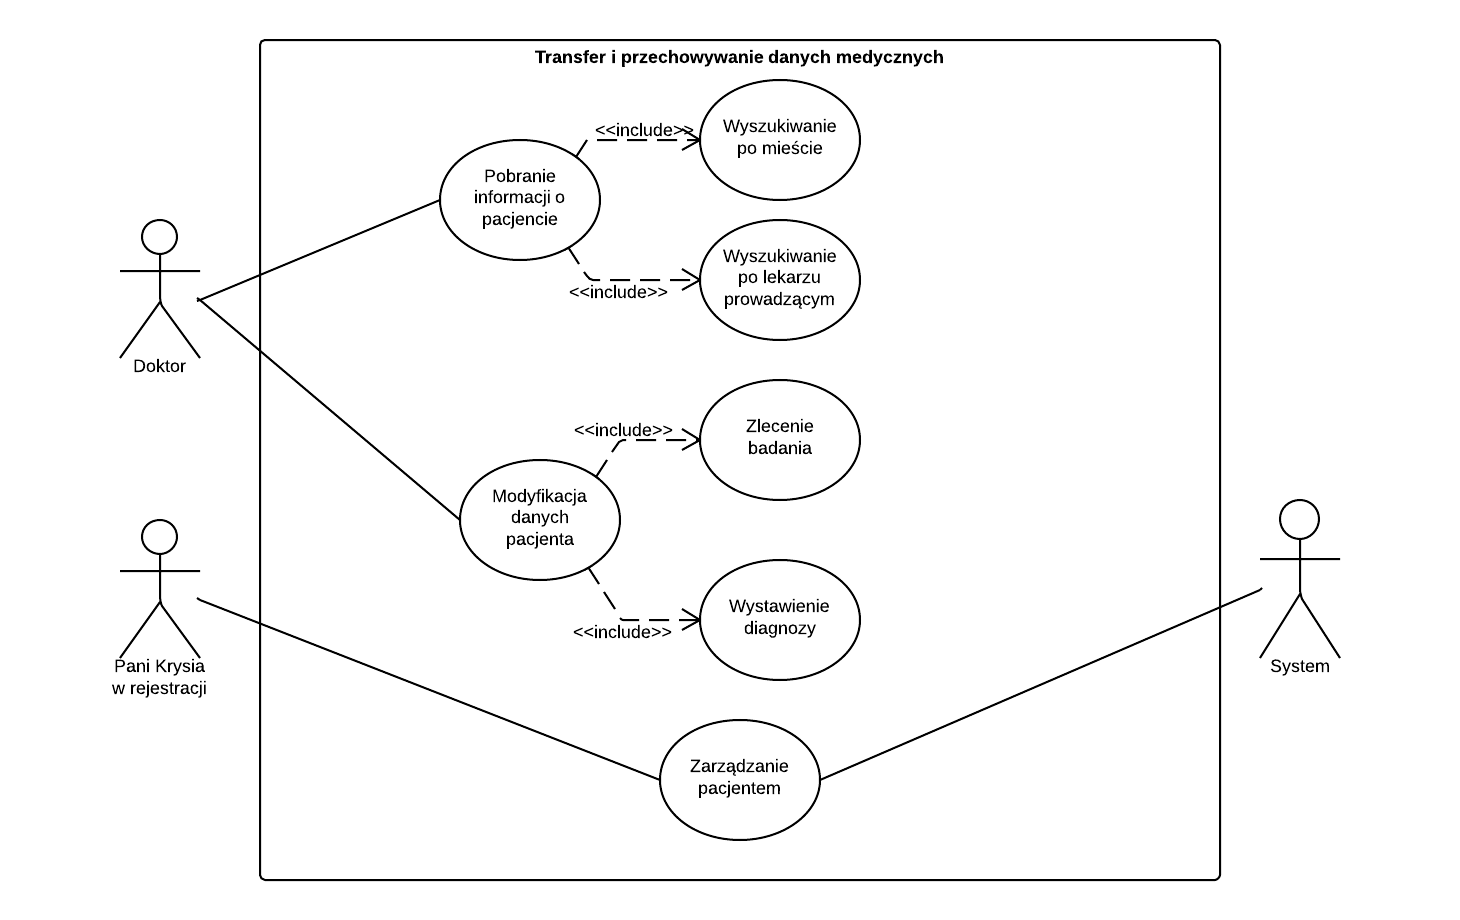
\includegraphics[width=\textwidth]{pics/UseCase}
	\caption{Diagram przypadków użycia}
	\label{fig:usecase}
\end{figure}
\begin{multicols}{2}

\subsection{Pobranie informacji o pacjencie}
\label{cha:patientinfo-usecase}

\subsubsection{Opis}
Przypadek użycia \quotedblbase Pobranie informacji o pacjencie\textquotedblright (Rys. \ref{fig:usecase}) przedstawia jedną z możliwych interakcji klienta (w tym wypadku lekarza) z systemem. Klient ma możliwość przefiltrowania pacjentów wg. miast i lekarzy prowadzących (lekarz może mieć pacjentów w róznych miastach).

\subsubsection{Zapytania SPARQL}
Przykładowe zapytanie użyte do pobrania pacjentów z danego miasta:
\begin{lstlisting}
SELECT ?patient WHERE { ?patient hl7:livesIn hl7:Nazwa_miasta }
\end{lstlisting}

\subsubsection{Implementacja po strone klienta - JAVA}
Aplikacja kliencka umożliwia pobranie listy pacjentów, parametryzowane wybranym miastem (poprzez pole select).
W analogiczny sposób można dodawać nowe funkcjonalności -  dodając nowe elementy interfejsu i przypisując odpowiednie zapytania SPARQL.

\section{SPARQL - zastosowanie}
\label{cha:wykorzystanie}

Poniżej zamieszczone są przykładowe zapytania sparql do pobierania informacji z grafów przedstawionych na rysunku 1 i rysunku 2.

\subsubsection{Wyszukiwanie węzłów-rodzeństw (poprzez użycie \quotedblbase relacji sameAs\textquotedblright }

Zapytanie:
\begin{lstlisting}
PREFIX rdf:     <http://www.w3.org/ 1999/02/22-rdf-syntax-ns#> 
PREFIX rdfs:    <http://www.w3.org/ 2000/01/rdf-schema#>
PREFIX owl:     <http://www.w3.org/ 2002/07/owl#>
PREFIX HL7: <http://sim.ontology/HL7#>
SELECT ?subject ?object
	WHERE { ?subject owl:sameAs ?object }
\end{lstlisting}

Wynik:
\begin{lstlisting}
{
  "head": {
    "vars": [ "subject" , "object" ]
  } ,
  "results": {
    "bindings": [
      {
        "subject": { "type": "uri" , "value": "http://sim.ontology/ HL7#Krakow" } ,
        "object": { "type": "uri" , "value": "http://sim.ontology/ HL7#Warszawa" }
      } ,
      {
        "subject": { "type": "uri" , "value": "http://sim.ontology/ HL7#Marek_Kendziorek" } ,
        "object": { "type": "uri" , "value": "http://sim.ontology/ HL7#Wojciech_Inglot" }
      } ,
      {
        "subject": { "type": "uri" , "value": "http://sim.ontology/ HL7#Patryk_Bak" } ,
        "object": { "type": "uri" , "value": "http://sim.ontology/ HL7#Wojciech_Inglot" }
      } ,
      {
        "subject": { "type": "uri" , "value": "http://sim.ontology/ HL7#Mazowsze" } ,
        "object": { "type": "uri" , "value": "http://sim.ontology/ HL7#Malopolska" }
      } ,
      {
        "subject": { "type": "uri" , "value": "http://sim.ontology/ HL7#Mazowsze" } ,
        "object": { "type": "uri" , "value": "http://sim.ontology/ HL7#Podkarpacie" }
      } ,
      {
        "subject": { "type": "uri" , "value": "http://sim.ontology/ HL7#Malopolska" } ,
        "object": { "type": "uri" , "value": "http://sim.ontology/ HL7#Podkarpacie" }
      }
    ]
  }
}

\end{lstlisting}







\subsubsection{Wyszukiwanie miast (węzły typu hl7:EntityCity) podrzędnych do węzła \quotedblbase Polska\textquotedblright, relacja: \quotedblbase isPartOf\textquotedblright }

Zapytanie:
\begin{lstlisting}
PREFIX rdf: <http://www.w3.org/ 1999/02/22-rdf-syntax-ns#>
PREFIX owl: <http://www.w3.org/ 2002/07/owl#>
PREFIX xsd: <http://www.w3.org/ 2001/XMLSchema#>
PREFIX rdfs: <http://www.w3.org/ 2000/01/rdf-schema#>
PREFIX hl7: <http://sim.ontology/HL7#>
SELECT ?subject
	WHERE {      
		?subject rdf:type hl7:EntityCity .
		?subject hl7:isPartOf hl7:Polska
	}
\end{lstlisting}

Wynik:
\begin{lstlisting}
{
  "head": {
    "vars": [ "subject" ]
  } ,
  "results": {
    "bindings": [
      {
        "subject": { "type": "uri" , "value": "http://sim.ontology/ HL7#Krakow" }
      } ,
      {
        "subject": { "type": "uri" , "value": "http://sim.ontology/ HL7#Warszawa" }
      }
    ]
  }
}


\end{lstlisting}

\subsubsection{Wyszukiwanie miasta w którym mieszka dana osoba}

Zapytanie:
\begin{lstlisting}
PREFIX rdf: <http://www.w3.org/ 1999/02/22-rdf-syntax-ns#>
PREFIX owl: <http://www.w3.org/ 2002/07/owl#>
PREFIX xsd: <http://www.w3.org/ 2001/XMLSchema#>
PREFIX rdfs: <http://www.w3.org/ 2000/01/rdf-schema#>
PREFIX hl7: <http://sim.ontology/HL7#>
SELECT ?city ?country
	WHERE {
		hl7:Wojciech_Inglot hl7:livesIn ?city .
		?city hl7:isPartOf ?region .
		?region hl7:isPartOf ?country
	           }
\end{lstlisting}

Wynik:
\begin{lstlisting}
{
  "head": {
    "vars": [ "city" , "country" ]
  } ,
  "results": {
    "bindings": [
      {
        "city": { "type": "uri" , "value": "http://sim.ontology/ HL7#Krakow" } ,
        "country": { "type": "uri" , "value": "http://sim.ontology/ HL7#Polska" }
      }
    ]
  }
}
\end{lstlisting}


\section{Podsumowanie}
\label{cha:podsumowanie}

Zaproponowana przez nas implementacja reprezentacji oraz transferu danych medycznych posiada wiele cech pożądanych przy projektowaniu tego typu systemów. Rozwiązanie to cechuje się bardzo dużą skalowalnoscią zarówno od strony wielkosci samego systemu jak i możliwosci rozbudowy przechowywanych w nim danych. Zastosowanie architektury typu SOA przy budowie systemu medyczneo pozwala na łatwą, modułową rozbudowę takiego systemu oraz ułatwioną integrację z innymi systemami medycznymi, zupełnie niezależnymi od siebie. Idąc dalej można skorzystać również z możliwosci oferowanych przez narzędzia jeszcze wyższych rzędów, takie jak szyny biznesowe, dzięki którym integracja mogłaby być jeszcze skuteczniejsza, nie naruszając jednoczesnie architektur oraz implementacji poszczególnych systemów.

W kwestii reprezentacji danych, wykorzystanie takiego frameworku jak Apache Jena pozwala na intuicyjne operowanie na dowolnej reprezentacji ontologii, ich rozbudowę w srodowisku programowania java, oraz ich graficzną reprezentację. Wykorzystanie tutaj w pracy srodowiska java jednoczesnie czyni znacznie prostszą integrację tego rozwiązania z opisanym wczesniej mechanizmem transferowania informacji, który również napisany jest w tym języku.
\end{multicols}

\begin{thebibliography}{1}

\bibitem{1}
Erik Sundvall, Mikael Nystrom, Daniel Karlsson, Martin Eneling, Rong Chen, Hakan Orman: Applying REST architecture to archetype-based electronic health record systems

\bibitem{2}
Wiesław Wajs, Krzysztof Rączka, Paweł Stoch, Piotr Kruczek: Integration Platform As Central Service Of Data Replication In Distributed Medical System

\bibitem{3}
Bartosz Jędrzejec: Pozyskiwanie wiedzy z dużych zbiorów danych z zastosowaniem adaptacyjnych procedur generowania zapytań, AGH Kraków 2008

\bibitem{4}
Dortje Loper, Meike Klettke, Livio Bruder, Andreas Heuer: Enabling flexible integration of healthcare information using entity-attribute-value storage model

\bibitem{5}
IHE cross-enterprise document sharing for imaging: interoperability testing software - Rita Noumeir, Berube Renaud - Springer Link database

\bibitem{6}
Integrating Clinical Trial Imaging Data Resources Using Service-Oriented Architecture and Grid Computing - Stefan Baumann El-Ghatta, Thierry Cladé, Joshua C. Snyder - Springer Link database

\bibitem{7}
Welcome to Health Information Science and Systems - Yanchun Zhang
LabKey Server: An open source platform for scientific data integration, analysis and collaboration - Elizabeth K Nelson, Britt Piehler - Springer Link database

\bibitem{8}
A database application for pre-processing, storage and comparison of mass spectra derived from patients and controls - Mark K Titulaer, Ivar Siccama - Springer Link database

\bibitem{9}
PASSIM – an open source software system for managing information in biomedical studies - Juris Viksna, Edgars Celms - Springer Link database

\bibitem{10}
The HL7 Clinical Document Architecture - Robert H Dolin, Liora Alschuler, Calvin Beebe; Journal of the American Medical Informatics Association Volume 8 Number 6

\bibitem{11}
The HL7 Clinical Document Architecture, Release 2 - Robert H Dolin, Liora Alschuler, Calvin Beebe; Journal of the American Medical Informatics Association Volume 13 Number 1

\bibitem{12}
HL7 Document Patient Record Architecture: An XML Document Architecture Based on a Shared Information Model - Robert H. Dolin, MD, Liora Alschuler, Fred Behlen, PhD, Paul V. Biron, MLIS, Sandy Boyer, RPh; Dan Essin, MD, Lloyd Harding, Tom Lincoln, MD, John E. Mattison, MD, Wes Rishel, Rachael Sokolowski, John Spinosa, MD, PhD, Jason P. Williams, MS

\bibitem{13}
HL7 Version 3—An object-oriented methodology for collaborative standards development - George W Beeler
A health-care data model based on the HL7 Reference Information Model - Eggebraaten, T.J.
Development of a Clinical Data Warehouse for Hospital Infection Control - Mary F Wisniewski, Piotr Kieszkowski, Brandon M Zagorski, 

\bibitem{14}
The HL7 Reference Information Model Under Scrutiny - Gunther Schadow , Charles N. Mead, D. Mead Walker
Biomedical Engineering (Chapter 19 - Toward Multi-Service Electronic Medical Records Structure) - Bilal I. Alqudah, Suku Nair

\bibitem{15}
Introduction to: HL7 Reference Information Model (RIM) - Health Level Seven International

\bibitem{16}
HL7 RIM: An Incoherent Standard - Barry Smith, Werner Ceusters

\bibitem{17}
Redundancy in electronic health records corpora: analysis, impact on text mining performance and mitigation strategies - Raphael Cohen, Michael Elhadad, Noemie Elhadad

\bibitem{18}
Initial experience with asynchronous transfer mode for use in medical imaging network - Minh Dovan, Louis M. Humphrey, Geri Cox, Carl E. Ravin

\bibitem{19}
A database application for pre-processing, storage and comparison of mass spectra derived  from patients and controls - Mark T Titulaer, Ivar Siccama, Lennard J Dekker

\bibitem{20}
Adding HL7 version 3 data types to PostgreSQL - Yeb Havinga, Willem Dijkstra, Ander de Keijzer

\bibitem{21}
Clinical data integration of distributed data sources using Health Level Seven (HL7) v3-RIM mapping - Teeradache Viangteeravat, Matthew N Anyanwu, Venkateswara Ra Nagisetty, Emin Kuscu, Mark Eijiro Sakauye, Duojiao Wu

\bibitem{22}
Electronic Medical Records vs. Electronic Health Records: Yes, There Is a Difference - Dave Garets and Mike Davis

\bibitem{23}
The “New” America Electronic Medical Record (EMR)—Design Criteria and Challenge - Ralph Grams

\bibitem{24}
Security of Medical Data Transfer and Storage in Internet. Cryptography, Antiviral Security and Electronic Signature Problems, which Must Be Solved in Nearest Future in Practical Context - Piotr Kasztelowicz, Marek Czubenko, Iwona Zięba

\bibitem{25}
Barriers to implement Electronic Health Records (EHRs) - Sima Ajami, Razieh Arab-Chadegani

\bibitem{26}
Holger Knublauch, Ray W. Fergerson, Natalya F. Noy and Mark A. Musen - The Protege OWL Plugin: An Open Development Environment for Semantic Web Applications

\end{thebibliography}

\end{document}